\subsubsection{Motor-Treiber}
Da man den Motor nicht direkt mit einem Raspberry steuern kann, braucht es einen Motortreiber. Der Twotrees DM542 5.6A Schrittmotortreiber\autocite{Treiber} ist ein leistungsstarker Treiber für 2-Phasen-Schrittmotoren, wie unser Motor, der verwendet wird. Hier ist eine kurze technische Produktbeschreibung:\\
\vspace{3mm}
Eigenschaften:
\begin{itemize}
    \item Leistung: Der Treiber unterstützt Motoren mit bis zu 5.6A Stromversorgung.
    \item Betriebsspannung: Geeignet für Gleichstromquellen im Bereich von 18-48V.
    \item Schrittauflösung: Präzise Mikroschrittsteuerung für genaue Positionierung.
    \item Phasen: Entwickelt für 2-Phasen-Schrittmotoren.
    \item Peak-Strom: Bietet einen Spitzenstrom von bis zu 4.2A für verbesserte Motorleistung.
\end{itemize}
\vspace{3mm}
Schutz und Zuverlässigkeit:
\begin{itemize}
    \item Überstromschutz: Der Treiber ist mit einem Überstromschutz ausgestattet, der den Motor vor Schäden durch zu hohe Ströme schützt.
    \item Wärmeschutz: Integrierter Schutzmechanismus gegen Überhitzung für eine zuverlässige Langzeitnutzung. So können wir die Tests lang genug durchführen.
\end{itemize}
Der Twotrees DM542 5.6A Schrittmotortreiber bietet eine leistungsstarke und zuverlässige Lösung für die Steuerung von 2-Phasen-Schrittmotoren in anspruchsvollen Anwendungen. Mit Funktionen wie Überstromschutz, Wärmeschutz und Mikroschrittsteuerung ist er eine geeignete Wahl für unsere Gyroskop Ansteuerung.
\begin{figure}[H]
    \centering
    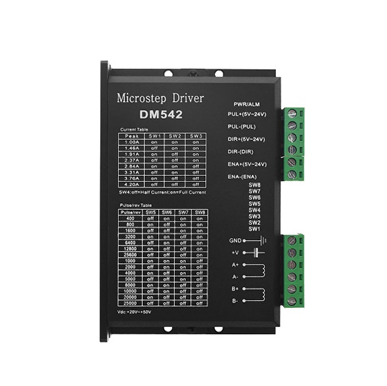
\includegraphics{image/treiber.png}
    \caption{Motor-Treiber}
    \label{fig:enter-label}
\end{figure}
